\documentclass{dmgt}

\usepackage{graphicx} % Required for inserting images
\usepackage[T1]{fontenc}
\usepackage[latin9]{inputenc} % Keep for compatibility with pdfLaTeX
\usepackage{float}
\usepackage{amsmath}
\usepackage{amsthm}
\usepackage{amssymb}
\usepackage{wasysym}
\usepackage{pdfpages}
\usepackage{verbatim}
\usepackage{multirow}
\usepackage{tikz}
\usepackage{caption}
\usepackage{subcaption}
\usepackage{amsfonts}
\usepackage{standalone}
\usepackage{multicol}
\usepackage{xcolor}

% TikZ settings
\usetikzlibrary{shapes, calc, positioning}
\tikzstyle{vertex}=[circle, draw, inner sep=2pt, minimum size=6pt]
\newcommand{\vertex}{\node[vertex]}

% Commands for Common Mathematical Fields and Number Sets
\newcommand{\kk}{\ensuremath{\Bbbk}} % Generic field symbol
\newcommand{\CC}{\ensuremath{\mathbb{C}}} % Complex numbers
\newcommand{\FF}{\ensuremath{\mathbb{F}}} % Field
\newcommand{\NN}{\ensuremath{\mathbb{N}}} % Natural numbers
\newcommand{\QQ}{\ensuremath{\mathbb{Q}}} % Rational numbers
\newcommand{\RR}{\ensuremath{\mathbb{R}}} % Real numbers
\newcommand{\ZZ}{\ensuremath{\mathbb{Z}}} % Integers

% Commands for Common Mathematical Sets and Spaces
\newcommand{\MM}{\ensuremath{\mathcal{M}}} % Set of matrices
\newcommand{\TT}{\ensuremath{\mathcal{T}}} % Topological space
\newcommand{\BB}{\ensuremath{\mathcal{B}}} % Basis or perhaps block
\newcommand{\VV}{\ensuremath{\mathcal{V}}} % Vector space
\newcommand{\WW}{\ensuremath{\mathcal{W}}} % Another vector space
\newcommand{\UU}{\ensuremath{\mathcal{U}}} % Another vector space
\newcommand{\PP}{\ensuremath{\mathcal{P}}} % Power set
\newcommand{\GG}{\ensuremath{\mathcal{G}}} % Fancy G

%% Required
%% \setarticle{1}{xx}{yyyy}

\newauthor{%
Bryan Freyberg}{%
B. Freyberg}{%
University of Minnesota Duluth\\
Duluth, MN, USA}[% 
frey0031@d.umn.edu]

\newauthor{%
Daniel Banegas}{%
D. Banegas }{%
University of Minnesota Duluth\\
Duluth, MN, USA}[% 
baneg003@d.umn.edu]

\title{Decomposition of complete graphs into forests with seven edges}

\keywords{Graph decomposition, forests, $\rho$-labeling}

\classnbr{05C51}

\begin{document}
\begin{abstract}
 Let $K$ be a graph and $G$ a subgraph of $K$. If $E(K)$ can be partitioned into edge-disjoint copies of $G$, we call the partition a $G$-decomposition of $K$ and say that $G$ decomposes $K.$ There are 47 forests with exactly 7 edges. We prove that every one decomposes the complete graph $K_{n}$ if and only if $n \equiv 0,1,7 \textrm{ or }8\pmod{14}.$

 
\end{abstract}
%%%%%%%%%%%5
\section{Introduction}
% Danny
%include a definition of cyclic decomposition and observe that only feasible for 0,1 mod 14\
A \textit{$G$-decomposition} of a graph $K$ is a set of mutually edge-disjoint subgraphs of $K$ which are isomorphic to a graph $G$. If such a set exists we say that $K$ \textit{allows} a $G$-decomposition, and if $K\cong K_{n}$ we sometimes call the decomposition a \textit{$G$-design of order $n$}.

$G$-decompositions are a longstanding topic in combinatorics, graph theory, and design theory, with roots tracing back to at least the 19th century. The work of Rosa and Kotzig in the 1960s on what are now known as graph labelings laid the foundation for the modern treatment of such problems. Using adaptations of these labelings alongside techniques from design theory, numerous papers have since been published on $G$-decompositions. This work is a natural continuation of Freyberg and Peters' recent paper on decomposing complete graphs into forests with six edges \cite{bib:Peters}. Their paper also includes a summary of $G$-decompositions for graphs $G$ with less than 7 edges.

Every connected component of a forest with 7 edges is a tree with 6 or less edges. All such trees are cataloged in Figure \ref{fig:catalog}. We use the naming convention $\mathbf{T_{j}^i}$ to denote the $i^{\textrm{th}}$ tree with $j$ vertices. For each tree $\mathbf{T_{j}^i}$, the names of the vertices, $v_t$ for $1 \leq t \leq j,$ will be used in the decompositions described in Section \ref{sec:7 or 8 mod 14}.

\begin{figure}[H]
    \centering
    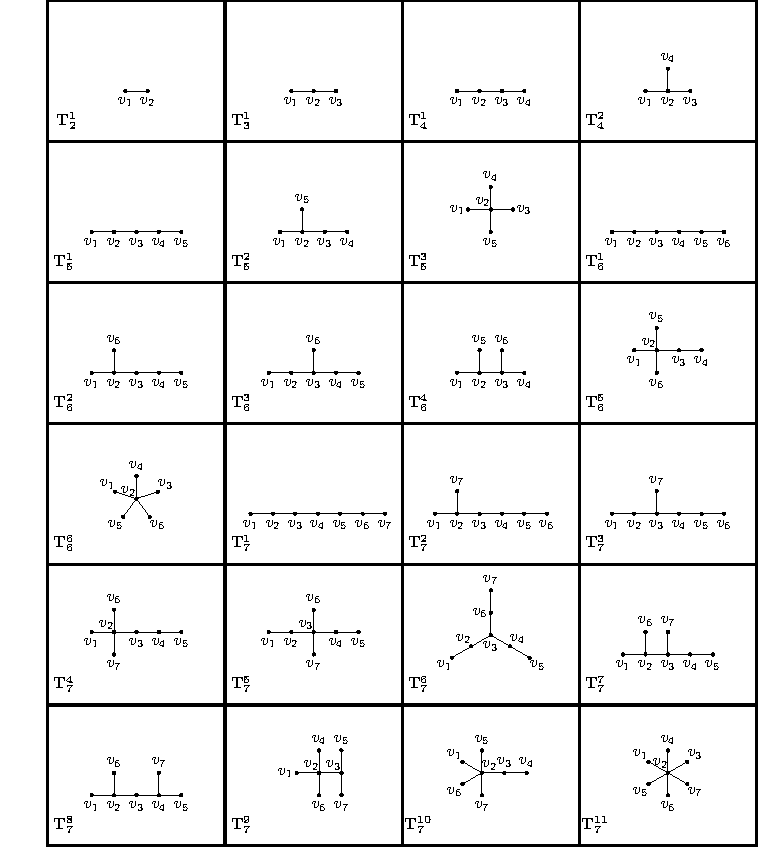
\includegraphics[]{tree chart.pdf}
    \caption{Trees with less than 7 edges}
    \label{fig:catalog}
\end{figure}

%%%%%%%%%%%%%%%%%%%%%%%%%%%%%%%%%%%%%%%%%
\section{$n \equiv 0 \textrm{ or } 1 \pmod{14}$}\label{sec:0 or 1 mod 14}
%Bryan text




\begin{dnt}[(Rosa \cite{bib:rosa})] \label{def:rho} 
 Let $G$ be a graph with $m$ edges.  A \textit{$\rho$-labeling} of $G$ is an injection $f: V(G) \rightarrow \{0,1,2, \dots, 2m\}$ that induces a bijective \textit{length function $\ell: E(G) \rightarrow \{1,2, \dots, m\}$} where 
    $$
    \ell(uv) = \text{min}\{|f(u)-f(v)|,2m+1-|f(u)-f(v)|\},
    $$
for all  $uv \in E(G)$.
\end{dnt}

Rosa showed that a $\rho$-labeling of a graph $G$ with $m$ edges and a cyclic $G$-decomposition of $K_{2m+1}$ are equivalent, which the next theorem shows. Later, Rosa, his students, and colleagues began considering more restrictive types of $\rho$-labeling to address decomposing complete graphs of more orders. Definitions of these labelings and related results follow.

\begin{theorem}[(Rosa \cite{bib:rosa})]\label{thm:Rhosa}  
Let $G$ be a graph with $m$ edges.  There exists a cyclic $G$-decomposition of $K_{2m+1}$ if and only if $G$ admits a $\rho$-labeling.
\end{theorem}

\begin{dnt}[(Rosa \cite{bib:rosa})] \label{def:sigma} 
A $\sigma$-labeling of a graph $G$ is a $\rho$-labeling such that $\ell(uv) = |f(u) - f(v)|$ for all $uv \in E(G).$
\end{dnt}

\begin{dnt}[(El-Zanati, Vanden Eynden \cite{cyclicbipart})] \label{def:rho and sigma ordered def} 
A $\rho$- or $\sigma$-labeling of a bipartite graph $G$ with bipartition $(A,B)$ is called an \emph{ordered} $\rho$- or $\sigma$-labeling and denoted $\rho^+,\sigma^+$, respectively, if $f(a) < f(b)$ for each edge $ab$ with $a \in A$ and $b \in B$.
\end{dnt}

\begin{theorem}[(El-Zanati, Vanden Eynden \cite{cyclicbipart})] \label{thm:rho plus} 
Let $G$ be a graph with $m$ edges which has a $\rho^+$-labeling.  Then $G$ decomposes $K_{2mk+1}$ for all positive integers $k$.
\end{theorem}

\begin{dnt}[(Freyberg, Tran \cite{tran})] \label{def:sigma plus minus} 
A $\sigma^{+-}$-\emph{labeling} of a bipartite graph $G$ with $m$ edges and bipartition $(A,B)$ is a $\sigma^+$-labeling with the property that $f(a) - f(b) \neq m$ for all $a \in A$ and $b \in B$, and $f(v) \not\in \{2m,2m-1\}$ for any $v\in V(G)$.
\end{dnt}

\begin{theorem}[(Freyberg, Tran \cite{tran})] \label{thm:sigma plus minus} 
Let $G$ be a graph with $m$ edges and a $\sigma^{+-}$-labeling such that the edge of length $m$ is a pendant. Then there exists a $G$-decomposition of both $K_{2mk}$ and $K_{2mk+1}$ for every positive integer $k$.
\end{theorem}

Figure \ref{fig:sigma} shows a $\sigma^{+-}$-labeling of every forest with 7 edges. These labelings along with Theorem \ref{thm:sigma plus minus} are enough to prove the following theorem. 
\begin{theorem}\label{thm:0 or 1 mod 14}
    Let $F$ be a forest with 7 edges. There exists an $F$-decomposition of $K_n$ whenever $n \equiv 0 \; \textrm{or} \; 1 \pmod{14}.$
\end{theorem}
\begin{proof}
    The proof follows from Theorem \ref{thm:sigma plus minus} and the labelings given in Figure \ref{fig:sigma}.
\end{proof}

%%%%%%%%%%%%%%%%
\section{$n \equiv 7 \textrm{ or } 8 \pmod{14}$} \label{sec:7 or 8 mod 14}
%Bryan text
% label tabels and do an example
\begin{figure}[H]
    \centering
    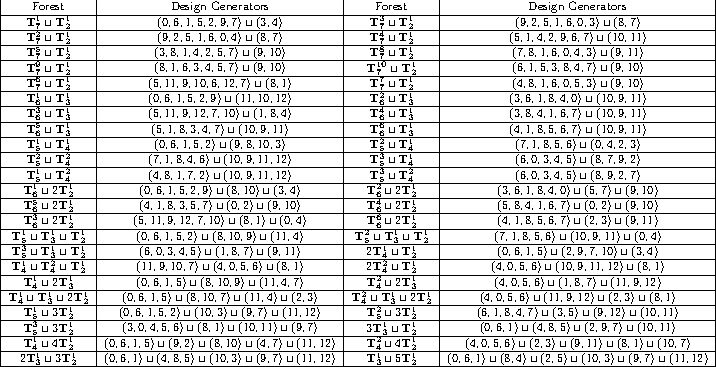
\includegraphics[scale=1.1]{0,1(mod 14).pdf}
    \caption{$\sigma^{+-}$-labelings for the forests with 7 edges}
    \label{fig:enter-label}
\end{figure}

\begin{exm}
    Danny's example
\end{exm}
%%%%%%%%%%%%%%%%
\section{$ G \cong K_{1,6} \cup K_2$}
%Danny

\begin{obs} \label{obs:K_n spec constr}
    Consider $\mathcal{K}=K_{t-1}$ for $t\geq 1$ whose nodes are $K_{14's}$. Clearly, $\mathcal{K}=K_{14(t-1)}$. So then $\mathcal{K}\lor K_{21}=K_{14(t-1)}\lor K_{21}=K_{14(t-1)+21}=K_{14t+7}$. Similarly $\mathcal{K}\lor K_{22}=K_{14t+8}$.
\end{obs}

\begin{obs}\label{obs:K_i,j spec constr}
    Consider $\mathcal{K}_{b}=K_{i:j}$ for $i,j\in \mathbb{N}$ whose nodes are $\overline{K}_{7}\,'s$. Clearly $\mathcal{K}=K_{7i:7j}$. Suppose we replace $0 \leq a\leq i$ nodes of partite set $I$ in $\mathcal{K}$ with $\overline{K}_{8}\,'s$. Then the resulting graph will be $K_{7(i-a)+8a:7j}$. The same holds if performed in partite set $J$.
\end{obs}

\begin{theorem}
Let $F=\mathbf{T_{6}^{11}}\sqcup\mathbf{T_{2}^{1}}$. If $F$ admits a $\sigma^{+-}$ labeling of $F$ and there exists an $F-$decomposition of $K_{21},K_{22},K_{7:7},K_{8:7}$, then there exists an $F-$decomposition of $K_{14t+7}$ and $K_{14t+8}$ for all positive integers $t$.
\end{theorem}

\begin{proof}

Suppose $F$ admits a $\sigma^{+-}$ labeling of $K_{14}$ and that there exists an $F-$deco-$\newline$mposition of $K_{21},K_{22},K_{7:7},K_{8:7}$. Let $t\geq 1$ and $\mathcal{K}=K_{t-1}$ whose nodes are $K_{14}$'s as outlined in observation \ref{obs:K_n spec constr}.
\\

\noindent By observation \ref{obs:K_i,j spec constr}, if $F$ decomposes $K_{7:7}$, then it decomposes $K_{14:14}$ since the edges of $K_{14:14}$ can be expressed as four copies of the edges of $K_{7:7}$. $F$ also decomposes $K_{21:14}$ via six copies of the edges of $K_{7:7}$. Similarly, $F$ then decomposes $K_{22:14}$ via two copies of the edges of $K_{8:7}$ and four copies of the edges of $K_{7:7}$. Therefore, $F$ decomposes the edges between all nodes of $\mathcal{K}$. Furthermore, $F$ also decomposes $\overline{\mathcal{K}}\lor K_{21}$ as well as $\overline{\mathcal{K}}\lor K_{22}$ since their edges are just many copies of $K_{21:14}$ and $K_{22:14}$.
\\

\noindent Lastly, since $F$ admits a $\sigma^{+-}-$labeling, by theorem \ref{thm:sigma plus minus} it decomposes $K_{14t}$. So then $F$ decomposes the internal edges of the nodes of $\mathcal{K}$ which are just $K_{14}$'s. So then since $F$ internally decomposes the nodes of $\mathcal{K}$ as well as the edges between them along with all edges of $\overline{\mathcal{K}}\lor K_{21}$ and $\overline{\mathcal{K}}\lor K_{22}$, $F$ in fact decomposes $\mathcal{K}\lor K_{21}$ and $\mathcal{K}\lor K_{22}$ which we know to be $K_{14t+7}$ and $K_{14t+8}$ by observation \ref{obs:K_n spec constr}.

\end{proof}

\begin{theorem}
    $\mathbf{T_{6}^{11}}\sqcup\mathbf{T_{2}^{1}}$ decomposes $K_{21}$ and $K_{22}$.
\end{theorem}

\begin{proof}
    See table $4$.
\end{proof}
\newpage
\begin{theorem}
    $\mathbf{T_{6}^{11}}\sqcup\mathbf{T_{2}^{1}}$ decomposes $K_{n,7}$ for all $n\geq 2$.
\end{theorem}

\begin{proof}
    Take the partite set of $n$ nodes to be $\ZZ_{n}$ and color them blue. Then, take the other partite set of $7$ nodes to be $\ZZ_{7}$ and color them red. Notice that $|E(K_{n,7})|=|\ZZ_{j}\oplus \ZZ_{7}|=7n$. So let us refer to edges of $K_{n,7}$ as elements of $\ZZ_{n}\oplus \ZZ_{7}$ and vice versa. Note that since $n\geq 2, (1,0)\neq (0,0)$.
    \\
    
    \noindent Now, let $E_{i}= (i,0)+\{(0,0),(1,1),(1,2),\hdots,(1,6)\}$ for each $i\in \ZZ_{n}$ and $F_{i}$ be the subgraph induced by $E_{i}$. Since each $F_{i}$ contains a path $(i,0)$ which is vertex disjoint from the star centered at the blue $i+1$, it must be isomorphic to $\mathbf{T_{6}^{11}}\sqcup\mathbf{T_{2}^{1}}$.
    \\
    %note to self: originally I thought of E_i's as (i,0) + (\{(0,0)\}\cup [(1,0)+[\langle (0,1)\rangle\setminus \{(0,0)\}]])

    %the union expression at the end is messy. However, the point of using groups here is basically that when we use generator notation we can swallow things up to get simpler things in terms of generators and it works out nicely here.
    
    \noindent Suppose that there exist distinct $i,j\in \ZZ_{n}$ such that $E_{i}\cap E_{j}\neq \emptyset$. But then we have that $(i,0)=(j,0)$ or $(i+1,a)=(j+1,b)$ for some $a,b\in \ZZ_{7}$, which is impossible. So all distinct $E_{i}$'s are pairwise disjoint, and therefore all distinct $F_{i}$'s are pairwise edge-disjoint. Lastly, $\bigcup_{i\in \ZZ_{n}} E_{i}=\langle (1,0)\rangle + [\{(0,0)\}\cup [(1,0)+\langle (0,1)\rangle] \setminus \{(1,0)\}]=\langle (1,0)\rangle + \langle (0,1)\rangle = \langle (1,0),(0,1)\rangle = \ZZ_{n}\oplus \ZZ_{7}$. Therefore, $\bigcup_{i\in \ZZ_{n}} F_{i} = K_{n,7}$. 
    \\
    
    \noindent Thus, $\{F_{i}\mid i\in \ZZ_{n}\}$ is a $\mathbf{T_{6}^{11}}\sqcup\mathbf{T_{2}^{1}}-$decomposition of $K_{n,7}$. Furthermore, This decomposition is generated by clicking the blue nodes of $F_{0}$ by $1$.
    
\end{proof}

%%%%%%%%%%%
\begin{thebibliography}{20}

\bibitem{bib:rosa}
A. Rosa,
On certain valuations of the vertices of a graph,
In: Theory of Graphs (Intl. Symp. Rome 1966), Gordon and Breach, Dunod, Paris,
1967, 349--355.

\bibitem{rosa}
A. Rosa,
On certain valuations of the vertices of a graph,
In: Theory of Graphs (Intl. Symp. Rome 1966), Gordon and Breach, Dunod, Paris,
1967, 349--355.

\bibitem{tran}
B. Freyberg, N. Tran, 
Decomposition of complete graphs into bipartite unicyclic graphs with eight edges, 
\textit{J. Combin. Math. Combin. Comput.}, \textbf{114}, (2020), 133--142.

\bibitem{bib:Peters}
B. Freyberg, R. Peters, 
Decomposition of complete graphs into forests with six edges, 
\textit{Discuss. Math. Graph Theory}, In-press (34), (2024).
    
\bibitem{seven}
D. Froncek, M. Kubesa, 
Decomposition of complete graphs into connected unicyclic bipartite graphs with seven edges,
\textit{Bull. Inst. Combin. Appl.}, accepted.


\bibitem{cyclic}
S. I. El-Zanati, C. Vanden Eynden,
On Rosa-type labelings and cyclic graph decompositions,
\textit{Math. Slovaca}, \textbf{59}, 2009, 1--18.

\bibitem{cyclicbipart}
S. I. El-Zanati, C. Vanden Eynden,
On the cyclic decomposition of complete graphs into bipartite graphs,
\textit{Australas. J. Combin.}, \textbf{24}, 2001, 209--219.

\end{thebibliography}


\end{document}

